\documentclass{article}
\usepackage[english]{babel}
\usepackage{tikz}
\usepackage{tkz-euclide}
\usetikzlibrary{shapes,shapes.geometric,intersections,through}
\usepackage{pgfplots}


\begin{document}
\title{ASSIGNMENT 03}
\author{Muneeb Ahmad Sheikh}
\date{\today}
\maketitle

\begin{itemize}
\item{\textbf{Question:}}\\

\textit{Construct a triangle of sides:}\\

$
a=4,\\

\hspace{1 cm}b=5, and\\

\hspace{1 cm}c=6
$\\

\item{\textbf{Solution:}}\\

we're given with the sides of a triangle as,\\

$
\hspace{1 cm}a=4,\\

\hspace{1 cm}b=5, and\\

\hspace{1 cm}c=6
$\\

Now,\\

\textit{Steps of Construct are:}\\
$

1: Draw a line BC of length c=6.\\

2:Taking B as centre draw an arc at the distance of as a=4.\\

3:Taking C as centre draw an arc at the distance of as b=5.\\

4: Name the point where the two arcs meet as A.\\

5: Join AB and AC.\\

6: We will get the required triangle.\\
$\\

$

Now, using Latex-tikz  below is the required triangle.
$\\
 \\



\begin{center}
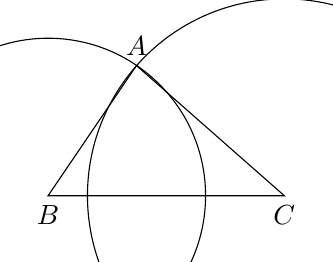
\begin{tikzpicture}[scale=.5]
\coordinate[label=below:$B$] (b) at (0,0);
\coordinate[label=below:$C$] (c) at (6,0);
\begin{pgfinterruptboundingbox}
\node(Cric1) at (b) [draw, circle through=($ (b) + (0:4) $)] {};
\node(Cric2) at (c) [draw, circle through=($ (c) + (0:5) $)] {};
\end{pgfinterruptboundingbox}
\coordinate[label=above:$A$] (a) at (intersection 2 of Cric1 and Cric2);
\draw(b)--(a)--(c)--cycle;
\end{tikzpicture}
\end{center}

\end{itemize}
\end{document}